\section{Results and Tests}

\subsection{Energy optimization}
Several methods for decreasing the power consumption of the program were implemented. We have focused on power consumption both when the program is idle and active. The eAprofiler in the Simplicity Studio bundle has been used to analyze the power consumption at various stages in the program.

\subsubsection{Idle}
In order to reduce power consumption during idle mode, the high frequency peripheral as well as the low energy oscillator are turned off, while the DAC being partly turned off. The CPU remains in deep sleep during this time. The output from the eAprofiler for the energy optimized program can be seen in figure 3, while the non-optimized program can be seen in figure 4. 


\begin{figure}[H]
  \centering
  % Trim er [left bottom right top]
  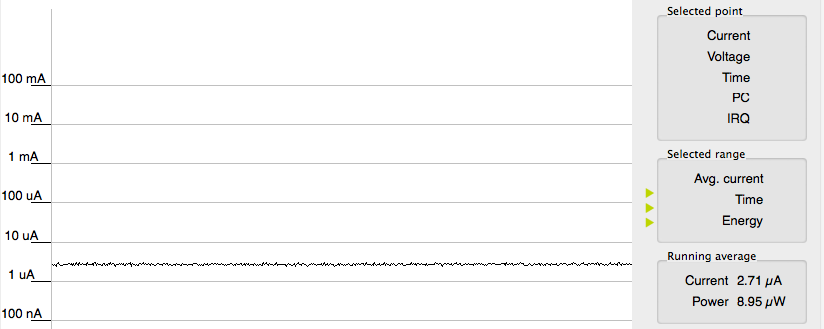
\includegraphics[clip, trim=0cm 0cm 0cm 0cm, width=12cm]{fig/idleEnergy.png}
  \caption{Low energy timer in idle mode}
\end{figure}

\begin{figure}[H]
  \centering
  % Trim er [left bottom right top]
  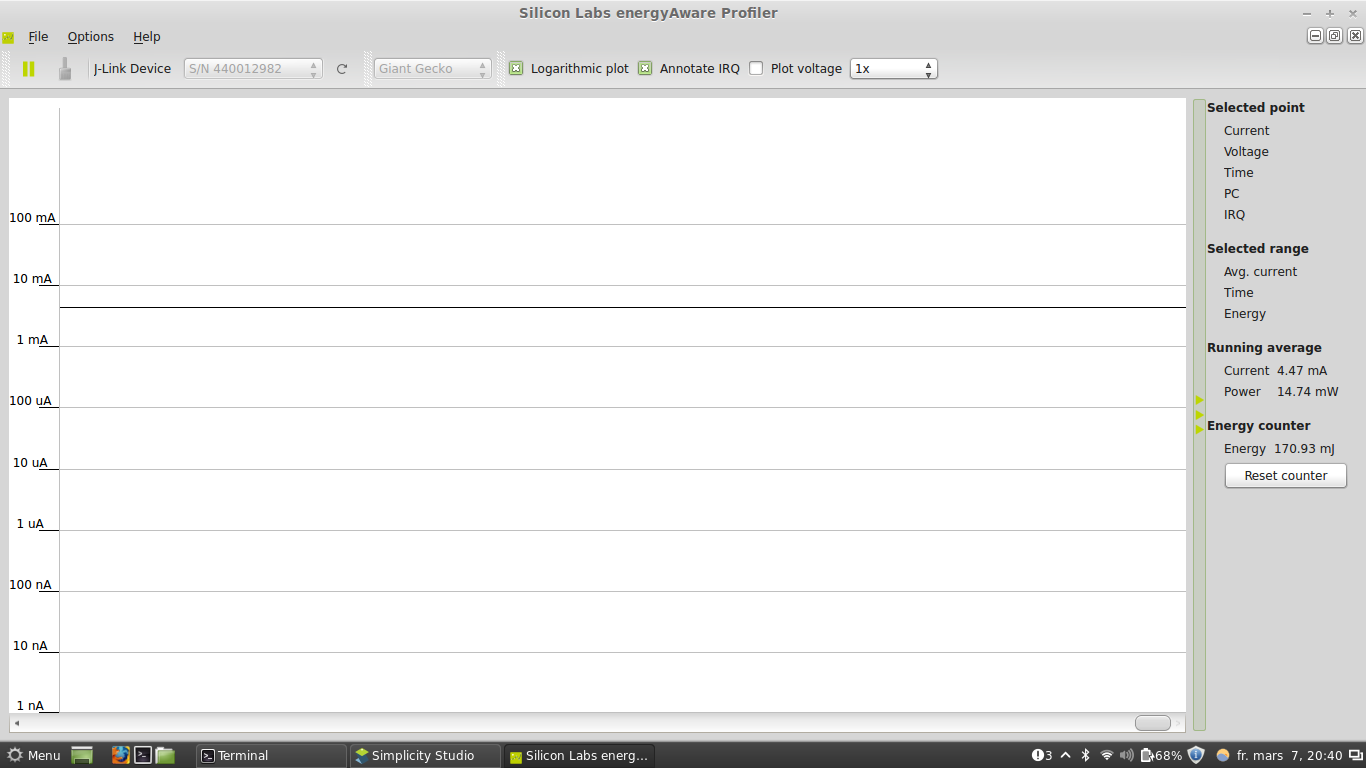
\includegraphics[clip, trim=0cm 0cm 0cm 0cm, width=12cm]{fig/Timer1Idle.png}
  \caption{Regular timer in idle mode}
\end{figure}


As seen the the energy usage is set at an comfortable level of 2.7 $\mu$A \\. This is significantly less than before the optimization, where the idle processor consumes 4.5 mA. 

\subsubsection{Running the syntheizer}
When the synthesiser is active, the CPU and the DAC is not utilised every clock cycle. It is possible to exploit this by disabling the CPU and the DAC between samples. The low energy timer is still active, but uses less energy compared to timer1. The energy consumption is illustrated in figure 5, while the non optimized program is illustrated in figure 6.    

\begin{figure}[H]
  \centering
  % Trim er [left bottom right top]
  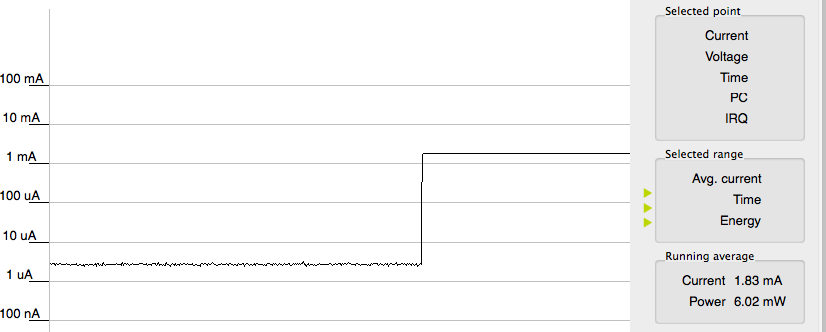
\includegraphics[clip, trim=0cm 0cm 0cm 0cm, width=12cm]{fig/marioEnergy.png}
  \caption{Low energy timer while running}
\end{figure}

\begin{figure}[H]
  \centering
  % Trim er [left bottom right top]
  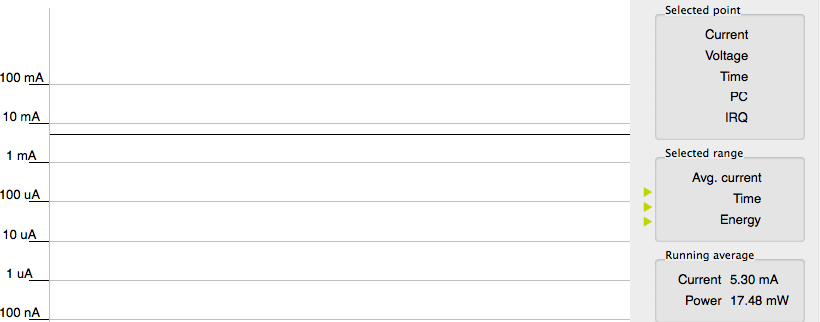
\includegraphics[clip, trim=0cm 0cm 0cm 0cm, width=12cm]{fig/playingWithoutOptimizations.png}
  \caption{Regular timer running without optimization}
\end{figure}


As seen by comparing the figures, the gains are significant when turning off the components during idle cycles. 


\subsubsection{Running with pre-computed samples}
When using pre-computed samples we use the same idea pointed out above. However, the result is slightly different. The number of idle cycles is increased, since the CPU does not need to perform expensive operations. This increases the time the CPU and DAC can spend in sleep mode, which reduces the overall energy consumption. This is shown in figure 7.

\begin{figure}[H]
  \centering
  % Trim er [left bottom right top]
  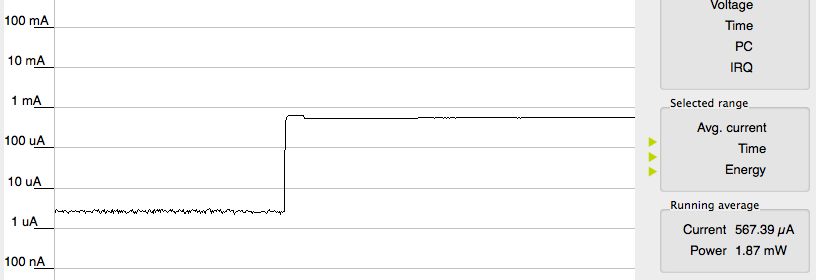
\includegraphics[clip, trim=0cm 0cm 0cm 0cm, width=12cm]{fig/energyBattlefield.png}
  \caption{Low energy timer while running Battlefield}
\end{figure}


As can be seen, the current hovers at around 614 $\mu$A, significantly lower than when using sound synthesizing.

\subsection{Sound functionality}

Our button setup was as follows:

\begin{table}[ht]
\caption{Buttons and corresponding melodies}
% title of Table
\centering
% used for centering table
\begin{tabular}{c c}
% centered columns (4 columns)
\hline
\hline %inserts double horizontal lines
Button & Melody \\ [0.5ex]
% inserts table
%heading
\hline
SW1 & Mario \\
SW2 & Shoot \\
SW3 & Hit dealt \\
SW4 & Hit received \\
SW5 & Battlefield intro \\
SW6-SW8 & Simple *beep*-noises \\
% [1ex] adds vertical space
\hline
%inserts single line%
\end{tabular}
\label{table:nonlin}
% is used to refer this table in the text
\end{table}

\subsubsection{Sound effects}

The sound effects were made by rapidly altering between the note macros defined in the sounds.h file. Three sound effects were created, which are the ones corresponding to SW2, SW3, and SW4. We were quite satisfied with these, as they were reminiscent of sound effects of old consoles and PC games from the early 1990s. The format of these can be viewed in the melodies.h-file.

\subsubsection{Mario}

For creating the super mario theme music, we initially used sound samples found online. However, we were not quite satisfied with these, as the sample periods were too short and the silence intervals too long. To fix this, a Python script was written to alter the samples by reducing the silence intervals by a certain factor, and increasing the sample periods by another factor. After a lot of trial and error, we ended up with a struct array of samples that we were reasonably satisfied with (this can be viewed in the melodies.h-file).

\subsubsection{Battlefield}

This is the intro music from the game Battlefield 1942. These samples were pre-computed, as described in the sound sampling section. 

\subsubsection{Tests}

Following are test cases created to firstly test whether the button input responds to expected sound output, and secondly, whether the energy levels behave as expected:



\emph{Input: } Press SW1-SW4\\
\emph{Expected output: } Play corresponding melody/sound effect with energy use of the sound synthesizer, then drop down to idle energy use when finished playing\\
\emph{Actual output: } as expected, with running energy use of 1.8 mA, and idle energy use of 2 $\mu$A \\


\emph{Input: } Press SW5\\
\emph{Expected output: } Play Battlefield with energy use of pre-computed samples, then drop down to idle energy use when finished playing\\
\emph{Actual output: } as expected with running energy use of 614 $\mu$A \\ and idle energy use of 2 $\mu$A \

\emph{Input: } Press SW6-SW8\\
\emph{Expected output: } Play simple *beep* sounds at different frequencies for a split second, then drop down to idle energy use when finished playing\\
\emph{Actual output: } as expected, with running energy use of 1.8 mA, and idle energy use of 2 $\mu$A \\

